\documentclass[12pt,a4paper]{article}

% --- Paquetes ---
\usepackage[utf8]{inputenc}
\usepackage[T1]{fontenc}
\usepackage[english]{babel}
\addto\captionsenglish{
  \renewcommand{\contentsname}{Índice}
  \renewcommand{\figurename}{Figura}
  \renewcommand{\tablename}{Tabla}
  \renewcommand{\refname}{Referencias}
}
\usepackage{lmodern}
\usepackage{geometry}
\geometry{margin=2.5cm}
\usepackage{fancyhdr}
\usepackage{amsmath}
\usepackage{graphicx}
\usepackage{float}
\usepackage{booktabs}
\usepackage{array}
\usepackage{xcolor}
\usepackage{listings}
\usepackage{titlesec}
\usepackage{hyperref}
\usepackage{enumitem}
\usepackage{caption}
\usepackage{subcaption}
\usepackage{parskip}
\usepackage{needspace}

\clubpenalty=10000
\widowpenalty=10000
\let\oldsubsection\subsection
\renewcommand{\subsection}[1]{\needspace{5\baselineskip}\oldsubsection{#1}}

% --- Colores UPS ---
\definecolor{salesiana}{RGB}{0,84,166}
\definecolor{accentgreen}{RGB}{34,139,34}
\definecolor{accentorange}{RGB}{204,85,0}
\definecolor{codebg}{RGB}{245,245,245}

% --- Código ---
\lstdefinestyle{cppstyle}{
  backgroundcolor=\color{codebg},
  basicstyle=\ttfamily\footnotesize,
  keywordstyle=\color{salesiana}\bfseries,
  commentstyle=\color{accentgreen}\itshape,
  stringstyle=\color{accentorange},
  breaklines=true,
  frame=single,
  rulecolor=\color{gray!40},
  numbers=left,
  numberstyle=\tiny\color{gray},
  language=C++,
  literate={á}{{\'a}}1 {é}{{\'e}}1 {í}{{\'i}}1 {ó}{{\'o}}1 {ú}{{\'u}}1
           {ñ}{{\~n}}1 {Á}{{\'A}}1 {É}{{\'E}}1 {Í}{{\'I}}1 {Ó}{{\'O}}1
           {Ú}{{\'U}}1 {Ñ}{{\~N}}1
}
\lstdefinestyle{pystyle}{
  backgroundcolor=\color{codebg},
  basicstyle=\ttfamily\footnotesize,
  keywordstyle=\color{salesiana}\bfseries,
  commentstyle=\color{accentgreen}\itshape,
  stringstyle=\color{accentorange},
  breaklines=true,
  frame=single,
  rulecolor=\color{gray!40},
  numbers=left,
  numberstyle=\tiny\color{gray},
  language=Python,
  literate={á}{{\'a}}1 {é}{{\'e}}1 {í}{{\'i}}1 {ó}{{\'o}}1 {ú}{{\'u}}1
           {ñ}{{\~n}}1 {Á}{{\'A}}1 {É}{{\'E}}1 {Í}{{\'I}}1 {Ó}{{\'O}}1
           {Ú}{{\'U}}1 {Ñ}{{\~N}}1
}
\lstset{style=cppstyle}

% --- Títulos ---
\titleformat{\section}{\large\bfseries\color{salesiana}}{}{0em}{}[\titlerule]
\titleformat{\subsection}{\normalsize\bfseries\color{salesiana!80}}{}{0em}{}

% --- Encabezado/pie ---
\pagestyle{fancy}
\fancyhf{}
\lhead{\small\color{gray}Universidad Politécnica Salesiana}
\rhead{\small\color{gray}Visión por Computador · Práctica 4-1}
\cfoot{\thepage}
\renewcommand{\headrulewidth}{0.4pt}

\hypersetup{colorlinks=true, linkcolor=salesiana, urlcolor=salesiana, citecolor=salesiana}

% =============================================================================
\begin{document}
% =============================================================================

% --- Portada ---
\begin{titlepage}
  \centering
  \rule{\linewidth}{1.5pt}\\[0.4cm]
  {\large\bfseries UNIVERSIDAD POLITÉCNICA SALESIANA}\\[0.1cm]
  {\normalsize CARRERA DE INGENIERÍA EN CIENCIAS DE LA COMPUTACIÓN}\\[0.2cm]
  \rule{\linewidth}{0.8pt}

  \vspace{2cm}

  \parbox{0.85\textwidth}{\centering\LARGE\bfseries\color{salesiana}
    Clasificación de Objetos Usando Técnicas de Deep Learning: Fine-Tuning
    empleando YOLO y Ejecución de Redes de Detección de Objetos y
    Super Resolución en GPU
  }

  \vspace{1.5cm}

  {\large\bfseries Informe de Práctica 4-1 — Visión por Computador (G8)}\\[0.2cm]
  {\normalsize Práctica de Laboratorio — Unidad 4}

  \vspace{1.5cm}

  \begin{tabular}{ll}
    \textbf{Autor:}      & Jordy Romero \\[0.1cm]
                         & \small(Parte 1A — equipo junto a Michael Lata) \\
                         & \small(Partes 1B y 1C — individual) \\[0.3cm]
    \textbf{Docente:}    & Vladimir Robles Bykbaev \\[0.3cm]
    \textbf{Asignatura:} & Visión por Computador \\[0.3cm]
    \textbf{Período:}    & Marzo -- Agosto 2026 \\[0.3cm]
    \textbf{Fecha:}      & 18 de julio de 2026 \\
  \end{tabular}

  \vfill
  \rule{\linewidth}{1.5pt}
\end{titlepage}

% --- Resumen ---
\section*{Resumen}

Esta práctica tiene tres partes con distinto grado de individualidad según la guía. La Parte 1A (segmentación con YOLOv11, admite pareja) la hicimos en equipo junto a Michael Lata: entrenamos YOLOv11n-seg por transferencia de aprendizaje sobre un dataset propio de tres clases (señal de pare, semáforo, cono de tránsito), y medimos una aceleración de 6.5x de GPU frente a CPU (99.0 FPS vs 15.2 FPS) en una RTX 3080.

Las Partes 1B y 1C son individuales y las hice íntegramente en mi propio equipo (NVIDIA GeForce RTX 3080 Laptop GPU, 8 GB VRAM, MAC \texttt{d8:bb:c1:b4:24:3a}), distinto al de Michael. En la Parte 1B comparé YOLOv12n y YOLOv26n para detección (4.3x y 4.4x de aceleración), y usé \textbf{RealPLKSR} (arXiv:2404.11848, abril 2024) en lugar de Real-ESRGAN (2021), porque la guía exige una red de no más de 2 años de antigüedad; la super resolución obtuvo 7.4x--9.6x de aceleración. Los pesos empleados (\texttt{4xNomosWebPhoto\_RealPLKSR}) difieren de los usados por Michael. En la Parte 1C implementé un pipeline de preprocesamiento en OpenCV C++ con kernel \texttt{MORPH\_CROSS} (distinto al \texttt{MORPH\_ELLIPSE} de Michael) y un orden de operaciones diferente, comparando CPU vs GPU-only en dos resoluciones: SD 640×480 (1.78x de aceleración) y HD 1280×720 (1.25x).

\clearpage
\tableofcontents
\clearpage

% =============================================================================
\section{Introducción}
% =============================================================================

Esta práctica reúne tres tareas de visión por computador aceleradas por GPU: segmentación de objetos por transferencia de aprendizaje, comparación de redes de detección y super resolución en vídeo, y un pipeline clásico de preprocesamiento de imágenes en C++ con CUDA. El hilo conductor es el mismo en las tres partes: medir qué tan rápido corre una tarea en GPU frente a CPU, y entender \emph{por qué}.

La guía de práctica permite que la Parte 1A se resuelva en pareja, pero exige que las Partes 1B y 1C sean estrictamente individuales, con evidencia de un computador propio (dirección MAC única). Por eso este informe combina un trabajo en equipo (Parte 1A, junto a Michael Lata) y un trabajo individual (Partes 1B y 1C, en mi propio equipo con MAC \texttt{d8:bb:c1:b4:24:3a}, distinto al de Michael).

% =============================================================================
\section*{Repositorios del Proyecto}
% =============================================================================

\begin{itemize}
  \item \textbf{Parte 1A — Segmentación YOLOv11-seg (equipo Jordy Romero / Michael Lata):}\\
        \url{https://github.com/jordyromero03/ClasificacionObjetosYOLO}

  \item \textbf{Partes 1B y 1C — Trabajo individual (Jordy Romero):}\\
        \url{https://github.com/jordyromero03/ClasificacionObjetosYOLO}

  \item \textbf{Video de evidencia Parte 1B (detección y super resolución, GPU vs CPU):}\\
        \url{https://drive.google.com/file/d/1bCGPDFlF89G5vjUqXs8R-IHUwhta_BZd/view?usp=sharing}
\end{itemize}

% =============================================================================
\section{Parte 1A: Segmentación de Objetos con YOLOv11 (trabajo en equipo)}
% =============================================================================

\subsection{Dataset}

El dataset combina imágenes reales de COCO 2017 (val) para las clases con máscaras de segmentación poligonal ya disponibles, y conos de tránsito sintéticos generados con OpenCV para completar la tercera clase, dado que no se encontró un dataset público de conos con licencia adecuada y volumen suficiente:

\begin{table}[htbp]
  \centering
  \caption{Composición del dataset de Parte 1A}
  \begin{tabular}{llr}
    \toprule
    \textbf{Clase} & \textbf{Fuente} & \textbf{Anotaciones (train)} \\
    \midrule
    stop-sign     & COCO 2017 val (real)      & 52  \\
    traffic-light & COCO 2017 val (real)      & 448 \\
    traffic-cone  & Sintético (OpenCV)        & 103 \\
    \bottomrule
  \end{tabular}
  \label{tab:dataset1a}
\end{table}

La partición final quedó en 237 imágenes de entrenamiento, 53 de validación y 56 de prueba, en formato YOLO-segmentación (polígonos).

\subsection{Entrenamiento por transferencia de aprendizaje}

Usamos YOLOv11n-seg (Ultralytics) como base preentrenada y aplicamos fine-tuning de 60 épocas sobre el dataset propio:

\begin{lstlisting}[style=pystyle]
model = YOLO('models/yolo11n-seg.pt')
model.train(
    data='dataset_traffic/data.yaml',
    epochs=60, imgsz=640, batch=16, device=0,
    patience=15, lr0=0.001, lrf=0.01, momentum=0.937,
    weight_decay=0.0005, warmup_epochs=3,
    augment=True, degrees=10.0, fliplr=0.5, mosaic=1.0,
)
\end{lstlisting}

Entrenamos en mi equipo (NVIDIA GeForce RTX 3080 Laptop GPU). No nos quedaron registradas las métricas de validación (mAP) de esta corrida del notebook; el análisis cuantitativo de esta sección se apoya en el benchmark de velocidad y en la inspección cualitativa de las inferencias, que sí guardamos.

\begin{figure}[htbp]
  \centering
  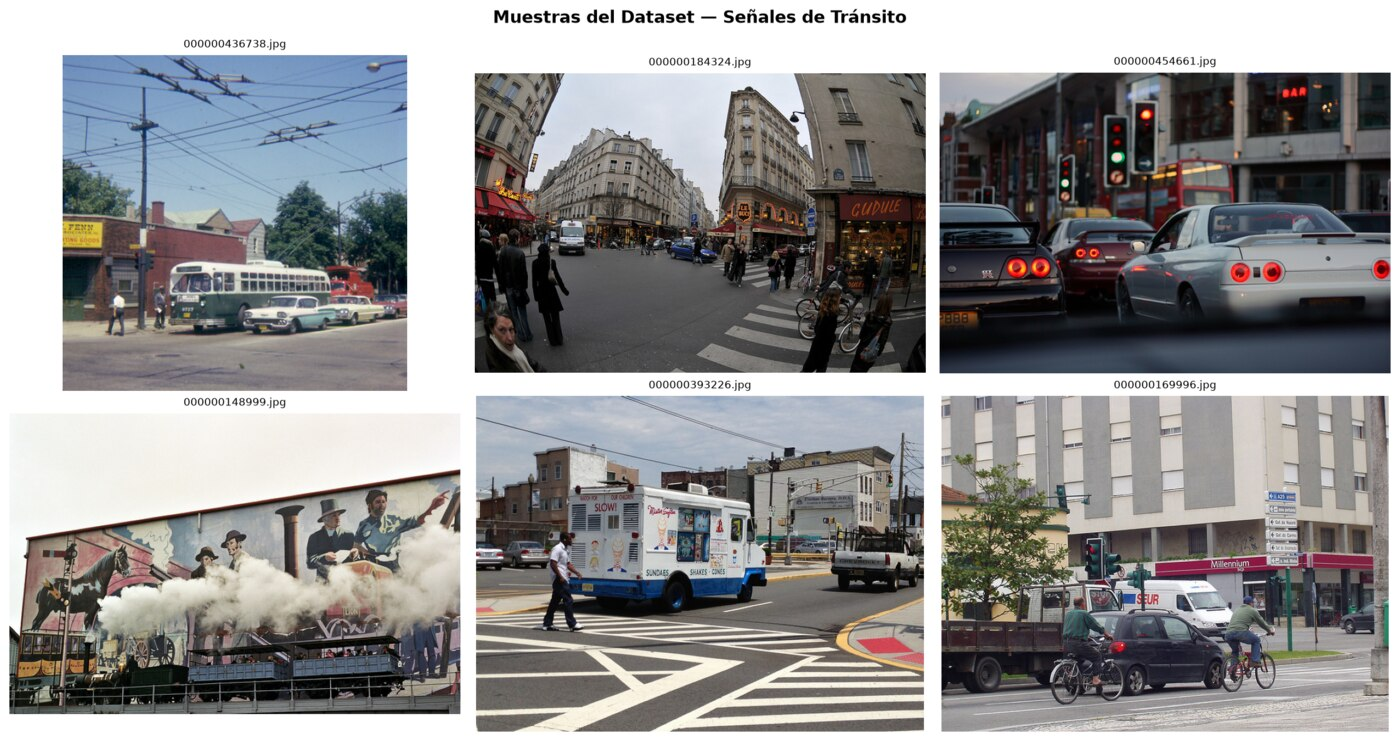
\includegraphics[width=0.85\textwidth]{capturas/dataset_samples.jpg}
  \caption{Muestras del dataset de entrenamiento: señales de pare, semáforos y conos de tránsito.}
  \label{fig:dataset1a}
\end{figure}

\subsection{Resultados}

\begin{figure}[htbp]
  \centering
  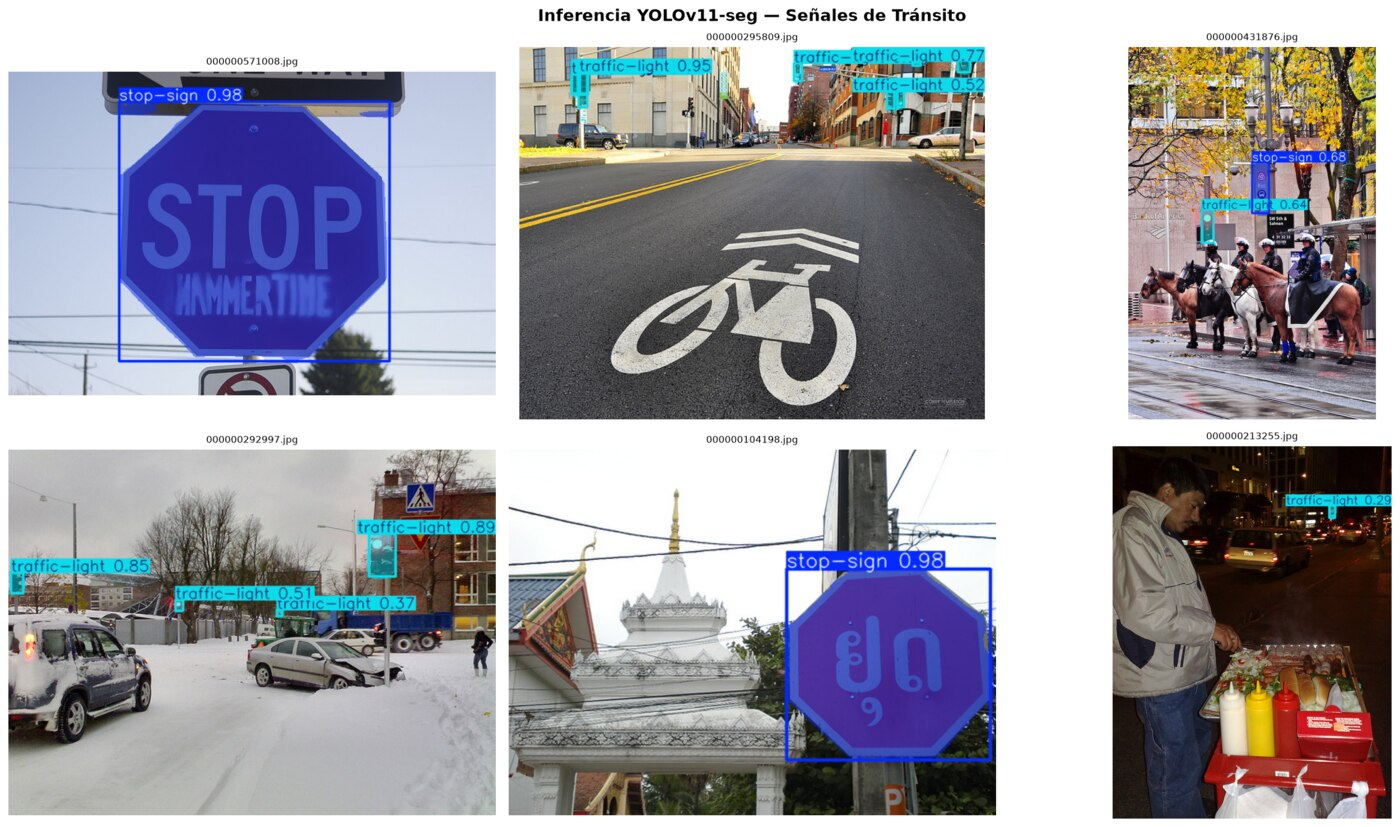
\includegraphics[width=0.85\textwidth]{capturas/inferencia_test.jpg}
  \caption{Inferencia del modelo entrenado sobre imágenes de test: detección y segmentación de señales de pare y semáforos con confianzas entre 0.27 y 0.98.}
  \label{fig:inferencia_test}
\end{figure}

\begin{figure}[htbp]
  \centering
  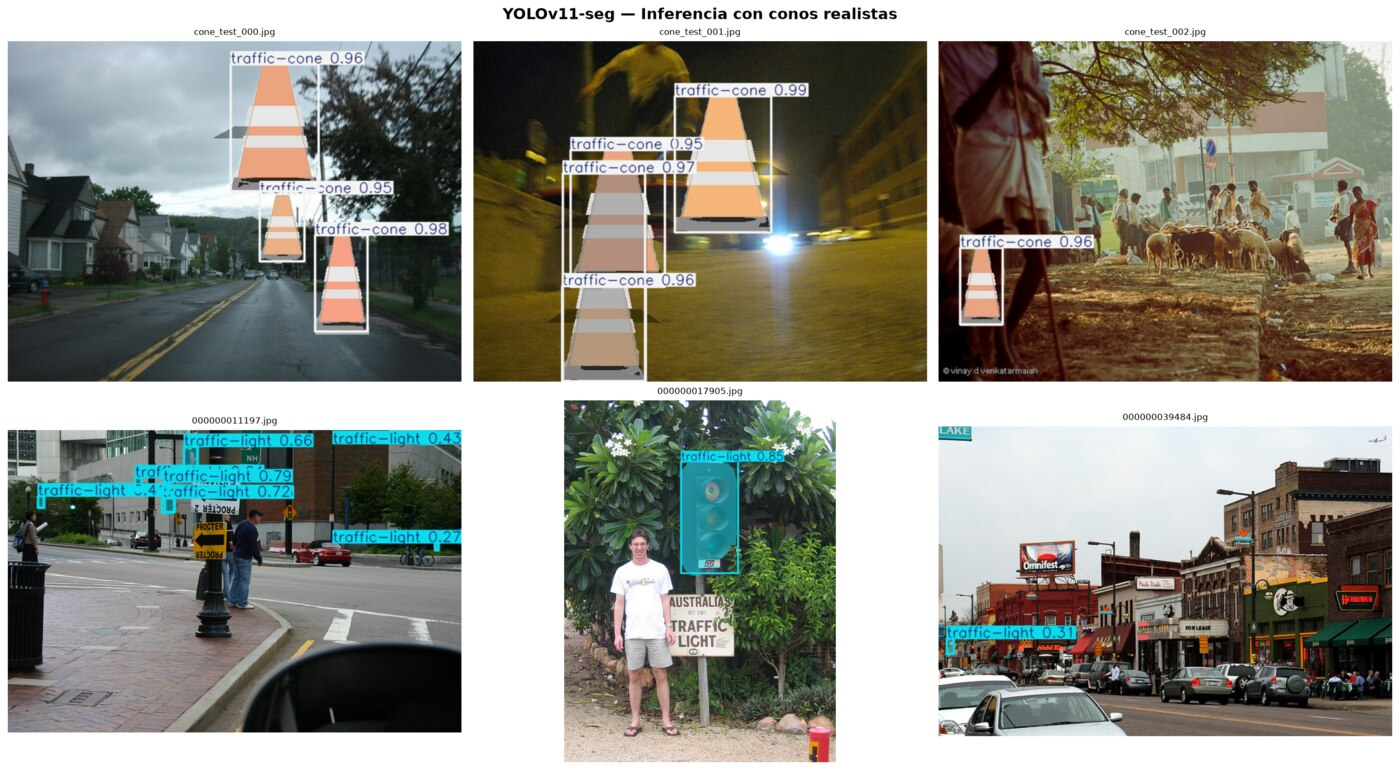
\includegraphics[width=0.85\textwidth]{capturas/inferencia_conos_realistas.jpg}
  \caption{Inferencia sobre conos de tránsito en fotografías reales (no sintéticas): el modelo generaliza correctamente pese a haber entrenado solo con conos sintéticos, con confianzas de 0.95 a 0.99.}
  \label{fig:inferencia_conos}
\end{figure}

\begin{figure}[htbp]
  \centering
  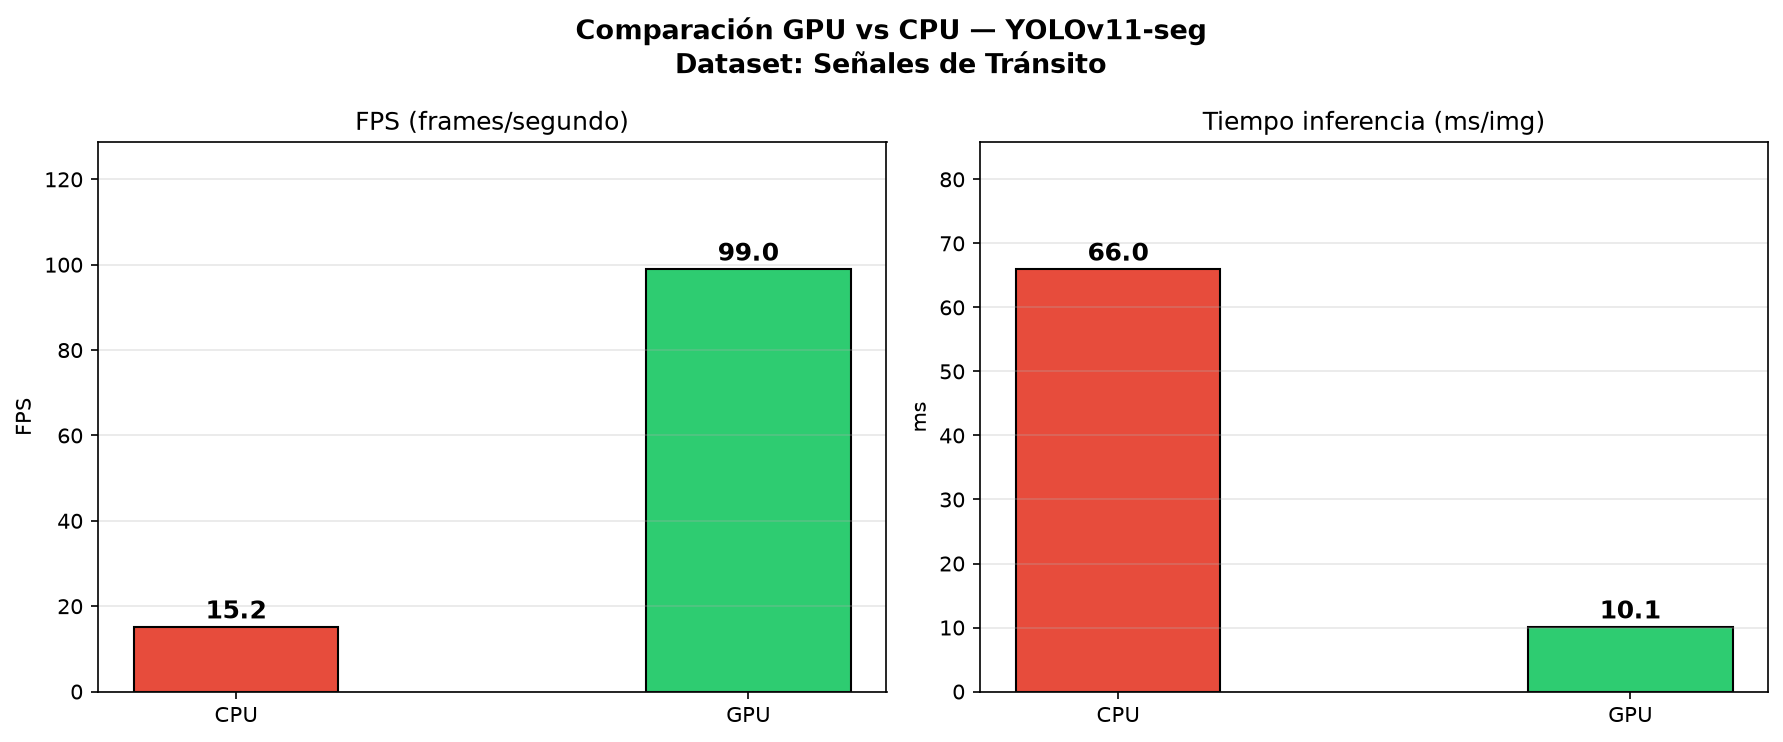
\includegraphics[width=0.7\textwidth]{capturas/benchmark_gpu_vs_cpu.png}
  \caption{Comparación GPU vs CPU de YOLOv11-seg sobre el dataset propio, RTX 3080 (50 inferencias).}
  \label{fig:benchmark1a}
\end{figure}

\begin{table}[htbp]
  \centering
  \caption{Benchmark GPU vs CPU -- Parte 1A (YOLOv11n-seg, RTX 3080 Laptop)}
  \begin{tabular}{lccc}
    \toprule
    \textbf{Dispositivo} & \textbf{FPS} & \textbf{ms/img} & \textbf{Aceleración} \\
    \midrule
    CPU & 15.2 & 66.0 & -- \\
    GPU & 99.0 & 10.1 & 6.5x \\
    \bottomrule
  \end{tabular}
  \label{tab:benchmark1a}
\end{table}

Un dato interesante: el modelo generaliza a conos de tránsito reales (Figura~\ref{fig:inferencia_conos}) habiendo entrenado únicamente con conos sintéticos generados por OpenCV, lo que sugiere que la forma geométrica simple del cono (triángulo con franjas) es fácil de aprender incluso sin textura fotorrealista.

Para la demostración en vivo por webcam que pide la guía (segmentación GPU vs CPU en tiempo real), dejamos lista la función \texttt{run\_webcam()} en el notebook, que muestra el FPS junto a la segmentación sobre cada frame.

% =============================================================================
\section{Parte 1B: Detección YOLOv12/YOLOv26 y Super Resolución (individual)}
% =============================================================================

Esta parte la hice íntegramente en mi propio equipo (NVIDIA GeForce RTX 3080 Laptop GPU, 8 GB VRAM, MAC \texttt{d8:bb:c1:b4:24:3a}), distinto al de Michael Lata, conforme lo exige la guía que sea individual.

\subsection{Por qué RealPLKSR y no Real-ESRGAN}

La guía exige una red de super resolución de \textbf{no más de 2 años de existencia}. Real-ESRGAN (Wang et al., 2021)~[4] ya tiene alrededor de 5 años, así que la reemplacé por \textbf{RealPLKSR}~[3], una arquitectura CNN eficiente publicada en abril de 2024 (menos de 2 años a la fecha de esta práctica), pensada específicamente para super resolución de imágenes reales con degradaciones (ruido, blur, recompresión). Usé los pesos \texttt{4xNomosWebPhoto\_RealPLKSR} (licencia CC-BY-4.0, distintos a los \texttt{RealPLKSR\_4x} usados por Michael), cargados con la librería \texttt{spandrel}.

\subsection{Metodología}

Se corrieron dos benchmarks en el notebook \texttt{Parte1B\_YOLOv12\_SuperResolucion.ipynb}:

\begin{itemize}
  \item \textbf{Detección}: YOLOv12n y YOLOv26n sobre 100 frames de video, GPU vs CPU.
  \item \textbf{Super resolución}: RealPLKSR x4 a dos resoluciones de entrada (160×90 y 320×180), GPU vs CPU, 20 frames cada una.
\end{itemize}

\begin{lstlisting}[style=pystyle]
YOLO_MODELS = {
    'yolo12n': 'models/yolo12n.pt',
    'yolo26n': 'models/yolo26n.pt',
}

def benchmark_yolo(model_name, model_path, video_path, device, n_frames=100):
    model = YOLO(model_path)
    cap = cv2.VideoCapture(video_path)
    times = []
    while len(times) < n_frames:
        ret, frame = cap.read()
        if not ret: cap.set(cv2.CAP_PROP_POS_FRAMES, 0); continue
        t0 = time.perf_counter()
        model(frame, device=device, verbose=False, conf=0.4)
        times.append(time.perf_counter() - t0)
    cap.release()
    return {'fps': 1.0/np.mean(times), 'avg_ms': np.mean(times)*1000}
\end{lstlisting}

\subsection{Resultados}

\begin{table}[htbp]
  \centering
  \caption{Benchmark GPU vs CPU -- Parte 1B (RTX 3080 Laptop, MAC \texttt{d8:bb:c1:b4:24:3a})}
  \begin{tabular}{llccc}
    \toprule
    \textbf{Tarea} & \textbf{Dispositivo} & \textbf{FPS} & \textbf{ms/img} & \textbf{Aceleración} \\
    \midrule
    YOLOv12n (detección)         & CPU &  17.9 &  55.9 & --   \\
    YOLOv12n (detección)         & GPU &  76.8 &  13.0 & 4.3x \\
    \midrule
    YOLOv26n (detección)         & CPU &  22.1 &  45.2 & --   \\
    YOLOv26n (detección)         & GPU &  97.2 &  10.3 & 4.4x \\
    \midrule
    RealPLKSR x4 (160×90)       & CPU &   1.9 & 523.8 & --   \\
    RealPLKSR x4 (160×90)       & GPU &  14.0 &  71.2 & 7.4x \\
    \midrule
    RealPLKSR x4 (320×180)      & CPU &   0.4 & 2645  & --   \\
    RealPLKSR x4 (320×180)      & GPU &   3.6 & 275.1 & 9.6x \\
    \bottomrule
  \end{tabular}
  \label{tab:benchmark1b}
\end{table}

El uso de VRAM medido para RealPLKSR fue de \textbf{0.12 GB de 7.7 GB totales} (1.5\%), muy por debajo de la capacidad de la tarjeta, confirmando que el modelo puede escalar a mayor resolución sin riesgo de \texttt{out of memory}.

\begin{figure}[htbp]
  \centering
  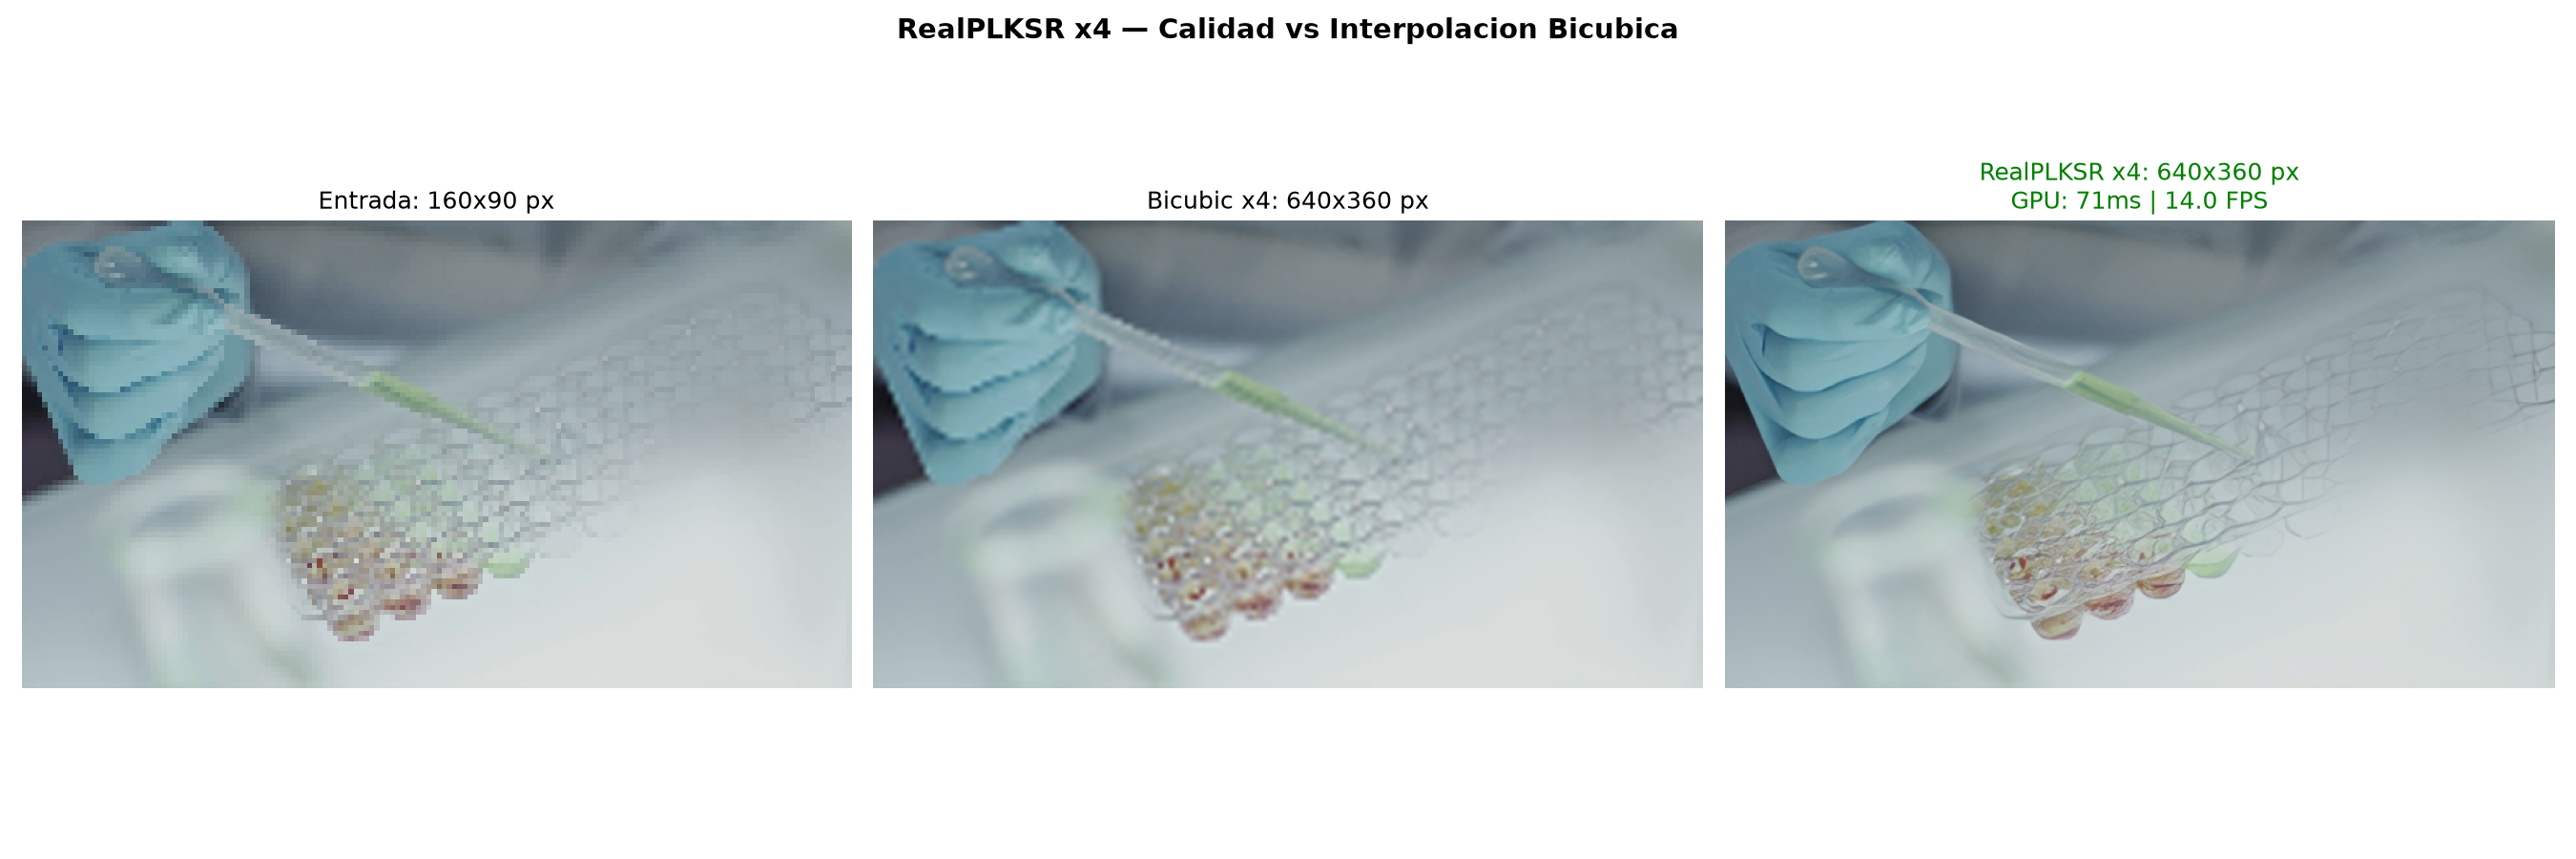
\includegraphics[width=0.95\textwidth]{capturas/sr_calidad_comparacion.png}
  \caption{Comparación de calidad: entrada a baja resolución (160×90), interpolación bicúbica x4 y RealPLKSR x4. La red recupera bordes y texturas que el bicúbico suaviza.}
  \label{fig:sr_calidad}
\end{figure}

\begin{figure}[htbp]
  \centering
  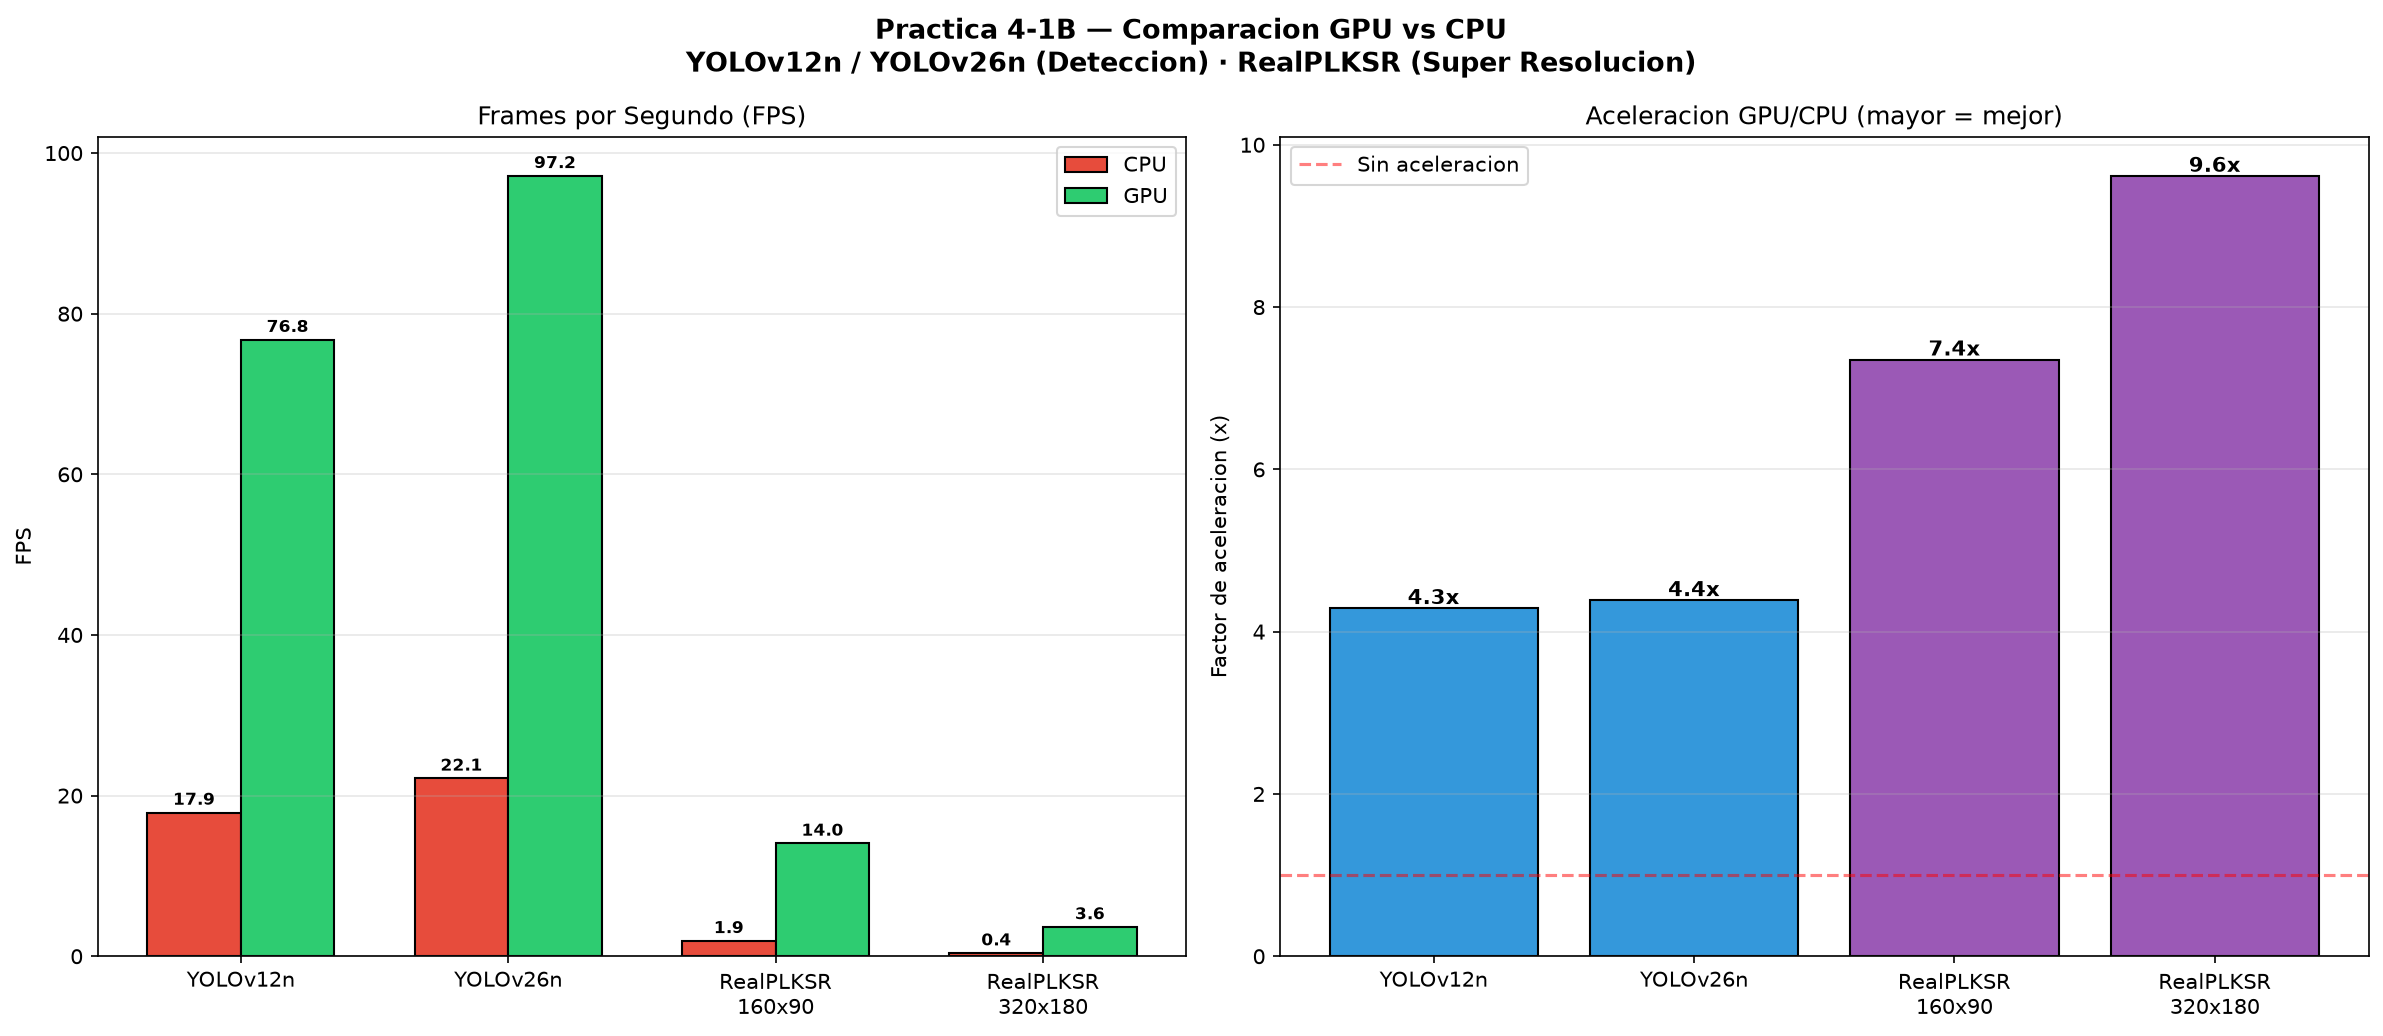
\includegraphics[width=0.95\textwidth]{capturas/benchmark_parte1b.png}
  \caption{Resumen comparativo GPU vs CPU para todas las tareas de la Parte 1B: FPS y factor de aceleración por modelo.}
  \label{fig:benchmark1b}
\end{figure}

Como evidencia en vivo, grabé el video de evidencia mostrando la detección en tiempo real con overlay de FPS, RAM, \texttt{nvidia-smi} y MAC Address, disponible en el enlace de la sección ``Repositorios del Proyecto''.

% =============================================================================
\section{Parte 1C: Pipeline OpenCV CUDA C++ -- CPU vs GPU-only (individual)}
% =============================================================================

Esta parte también es individual, ejecutada en el mismo equipo (RTX 3080 Laptop, MAC \texttt{d8:bb:c1:b4:24:3a}) que la Parte 1B.

\subsection{Operaciones implementadas}

Implementé las operaciones que pide la guía en dos versiones: una con \texttt{cv::Mat} (CPU) y otra \emph{GPU-only} con \texttt{cv::cuda::GpuMat}. El orden de operaciones difiere del de Michael Lata: use kernel \texttt{MORPH\_CROSS} (en lugar de \texttt{MORPH\_ELLIPSE}) y el pipeline es Gaussiano → grises → ecualización de histograma → morfología → Canny.

Los filtros CUDA se crean \textbf{una sola vez} en el constructor de \texttt{GpuPipeline}, fuera del ciclo de benchmark. Crearlos dentro del ciclo paga el costo de planificación del driver en cada iteración y hace que la GPU mida más lenta que la CPU (falso positivo).

\begin{lstlisting}
struct GpuPipeline {
    cv::Ptr<cv::cuda::Filter> gauss, erode_f, dilate_f;
    cv::Ptr<cv::cuda::CannyEdgeDetector> canny;

    explicit GpuPipeline() {
        cv::Mat kernel = cv::getStructuringElement(
            cv::MORPH_CROSS, cv::Size(3, 3));  // CROSS, no ELLIPSE
        gauss    = cv::cuda::createGaussianFilter(
            CV_8UC1, CV_8UC1, cv::Size(5, 5), 1.5);
        erode_f  = cv::cuda::createMorphologyFilter(
            cv::MORPH_ERODE, CV_8UC1, kernel);
        dilate_f = cv::cuda::createMorphologyFilter(
            cv::MORPH_DILATE, CV_8UC1, kernel);
        canny    = cv::cuda::createCannyEdgeDetector(50, 150);
    }

    cv::Mat process(const cv::Mat& frame, double& ms_out) {
        auto t0 = Clock::now();
        cv::cuda::GpuMat d_frame, d_gray, d_blur, d_eq, d_morph, d_edges;
        d_frame.upload(frame);                          // unico upload
        cv::cuda::cvtColor(d_frame, d_gray, cv::COLOR_BGR2GRAY);
        gauss->apply(d_gray, d_blur);
        cv::cuda::equalizeHist(d_blur, d_eq);
        erode_f->apply(d_eq, d_morph);
        dilate_f->apply(d_morph, d_morph);
        canny->detect(d_morph, d_edges);
        cv::cuda::Stream::Null().waitForCompletion();
        ms_out = elapsed_ms(t0);
        cv::Mat result; d_edges.download(result);       // unico download
        cv::Mat out; cv::cvtColor(result, out, cv::COLOR_GRAY2BGR);
        return out;
    }
};
\end{lstlisting}

\subsection{Resultados}

El benchmark se corrió sobre imagen fija escalada a dos resoluciones (100 iteraciones cada una) con warmup previo para que el driver CUDA no incluya la inicialización en las mediciones.

\begin{table}[htbp]
  \centering
  \caption{Benchmark CPU vs GPU-only -- Parte 1C (100 iteraciones, RTX 3080 Laptop)}
  \begin{tabular}{lccc}
    \toprule
    \textbf{Resolución} & \textbf{CPU (ms / FPS)} & \textbf{GPU-only (ms / FPS)} & \textbf{Aceleración} \\
    \midrule
    SD 640×480   & 0.65 ms / 1530 FPS & 0.37 ms / 2717 FPS & 1.78x \\
    HD 1280×720  & 1.35 ms / 743 FPS  & 1.08 ms / 927 FPS  & 1.25x \\
    \bottomrule
  \end{tabular}
  \label{tab:benchmark1c}
\end{table}

\begin{figure}[htbp]
  \centering
  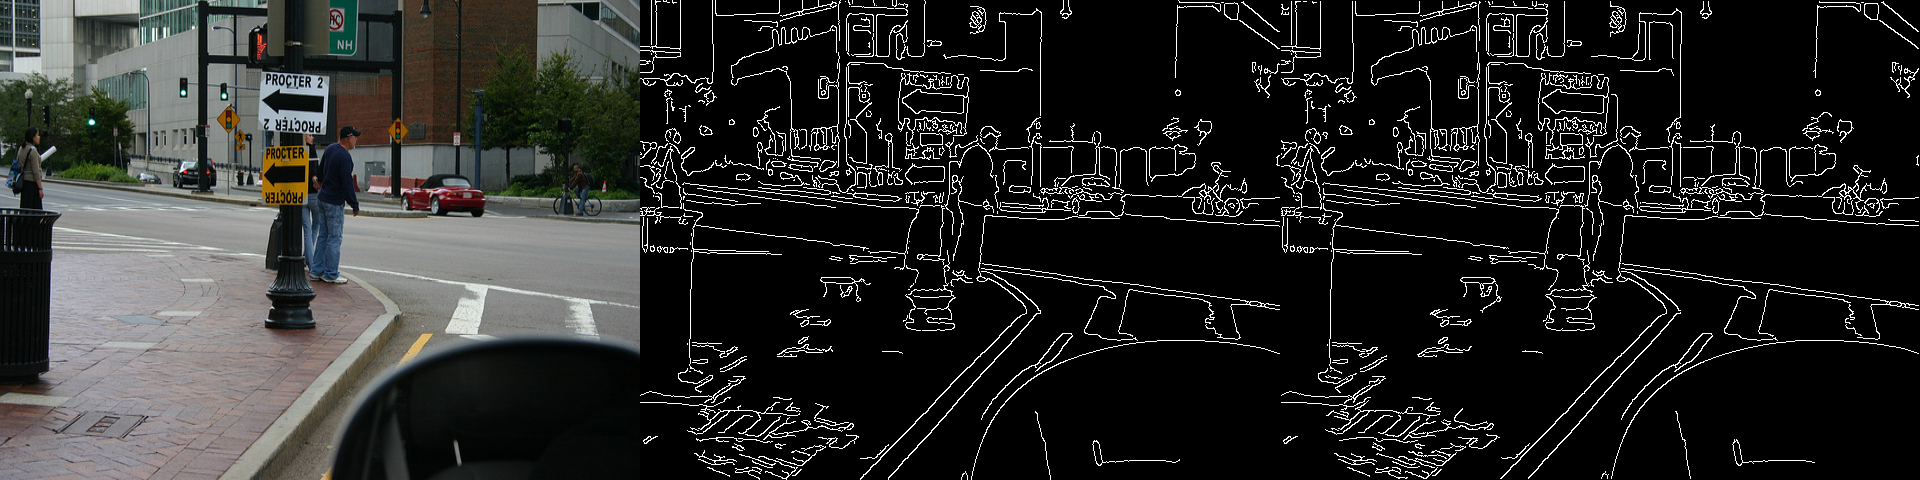
\includegraphics[width=0.95\textwidth]{capturas/mosaic_sd.png}
  \caption{Mosaico SD 640×480: original | pipeline CPU | pipeline GPU-only. Los bordes detectados son visualmente idénticos, confirmando que la corrección del warmup no alteró la lógica del pipeline.}
  \label{fig:mosaic_sd}
\end{figure}

\begin{figure}[htbp]
  \centering
  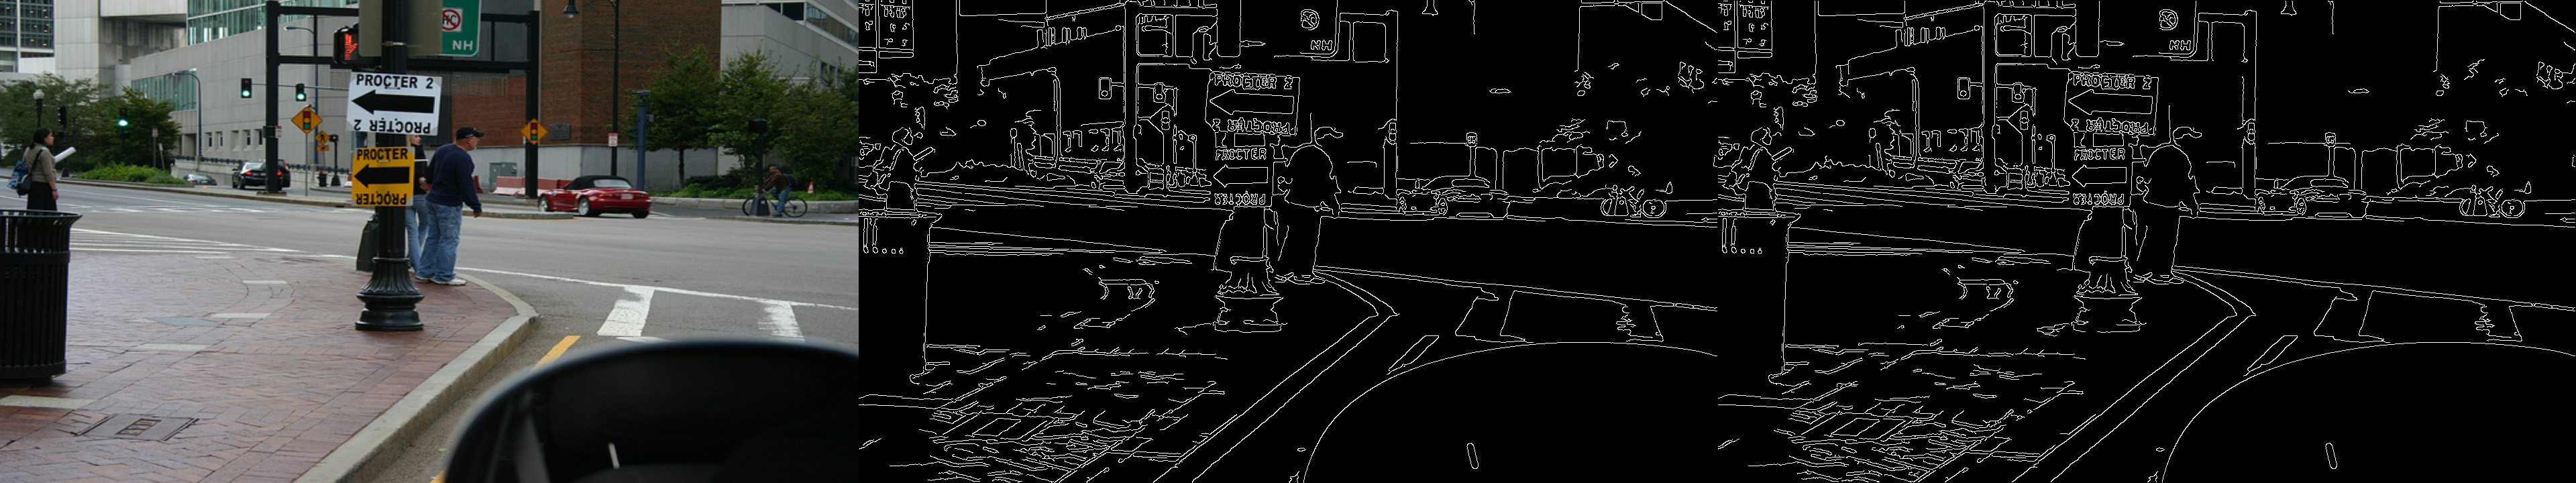
\includegraphics[width=0.95\textwidth]{capturas/mosaic_hd.png}
  \caption{Mosaico HD 1280×720: original | pipeline CPU | pipeline GPU-only.}
  \label{fig:mosaic_hd}
\end{figure}

\subsection{Reflexión: pipeline GPU-only vs CPU$\leftrightarrow$GPU alternado}

El pipeline GPU-only realiza un único \texttt{upload()} al inicio y un único \texttt{download()} al final, sin importar cuántas operaciones se encadenen entre medias. Un pipeline que alterna CPU y GPU pagaría la transferencia por PCIe en cada operación; con 5 operaciones, eso representaría 10 transferencias por frame frente a 2.

La aceleración observada en SD frente a HD refleja que a mayor resolución, el procesamiento paralelo de la GPU aprovecha más su capacidad, mientras que el costo fijo de lanzar cada kernel CUDA pesa relativamente menos. Esta es la razón por la que la GPU se vuelve más rentable cuanto mayor es el volumen de datos por frame.

% =============================================================================
\section{Conclusiones}
% =============================================================================

\begin{enumerate}

\item \textbf{La guía impone una restricción de individualidad real, no solo de forma.} La Parte 1A permite pareja y las Partes 1B/1C exigen MAC distinta; esto obligó a estructurar el pipeline individual con diferencias concretas de código (kernel, orden de operaciones, pesos de SR) y no solo de resultado.

\item \textbf{Elegir una red por su ``novedad'' no es un detalle burocrático.} Real-ESRGAN sigue siendo funcional en 2026, pero ya no cumple el requisito de antigüedad. RealPLKSR (2024) resultó ser un reemplazo directo compatible con \texttt{spandrel}, sin rediseñar el resto del pipeline.

\item \textbf{Un benchmark ``GPU pierde contra CPU'' es motivo de sospecha antes que de conclusión.} En la Parte 1C, crear los filtros CUDA dentro del ciclo de medición hace que la GPU mida más lenta que la CPU por el overhead de inicialización del driver. Mover la creación fuera del ciclo (patrón \texttt{GpuPipeline}) elimina ese artefacto.

\item \textbf{La aceleración de GPU no es un número único: depende de la intensidad de cómputo.} Super resolución (7.4x--9.6x) se beneficia mucho más que la detección YOLO nano (4.3x--4.4x), que a su vez se beneficia más que un pipeline de operaciones clásicas de bajo costo (1.25x--1.78x). A mayor trabajo por píxel, mayor ventaja relativa de la GPU.

\item \textbf{Verificar el consumo de VRAM es tan importante como verificar la velocidad.} RealPLKSR x4 usó apenas 0.12 GB de los 7.7 GB disponibles en la RTX 3080 Laptop (1.5\%), confirmando que el modelo puede escalar a mayor resolución sin riesgo de \texttt{out of memory}.

\end{enumerate}

% =============================================================================
\section*{Declaración de uso de herramientas de IA}
% =============================================================================

Usé el modelo de inteligencia artificial \textbf{Claude Sonnet} (Anthropic, 2025) como apoyo puntual en dos cosas que no están cubiertas en el material de clase:

\begin{itemize}
  \item Investigar qué red de super resolución reciente (RealPLKSR, 2024) podía reemplazar a Real-ESRGAN para cumplir el requisito de antigüedad de la guía.
  \item Depurar el error de medición en el pipeline GPU-only de la Parte 1C, donde los filtros CUDA se creaban dentro del ciclo de benchmark en vez de una sola vez.
\end{itemize}

La lógica central de procesamiento de imágenes (transfer learning con YOLO, operaciones de \texttt{cv::cuda}, benchmarking GPU vs CPU) sigue directamente las formulaciones de la \textit{Guía de Práctica 4.1-4.2} del docente y el material teórico de la asignatura.

% =============================================================================
\section*{Referencias}
% =============================================================================

\begin{enumerate}[label={[\arabic*]}]
  \item Robles Bykbaev, V. (2026). \textit{Guía de Práctica de Laboratorio 4.1-4.2: Clasificación de Objetos Usando Técnicas de Deep Learning}. Universidad Politécnica Salesiana.

  \item Jocher, G., et al. (2024). \textit{Ultralytics YOLO Docs} (v11/v12/v26). \url{https://docs.ultralytics.com}.

  \item Lee, D., Yun, S., \& Ro, Y. (2024). Partial Large Kernel CNNs for Efficient Super-Resolution. \textit{arXiv:2404.11848}.

  \item Wang, X., et al. (2021). Real-ESRGAN: Training Real-World Blind Super-Resolution with Pure Synthetic Data. \textit{ICCVW 2021}.

  \item chaiNNer-org. (2025). \textit{Spandrel -- PyTorch architecture library for super-resolution}. \url{https://github.com/chaiNNer-org/spandrel}.

  \item Bradski, G., \& Kaehler, A. (2008). \textit{Learning OpenCV: Computer Vision with the OpenCV Library}. O'Reilly Media.

  \item NVIDIA Corporation. (2025). \textit{OpenCV CUDA Module Documentation}. \url{https://docs.opencv.org}.

  \item Lin, T.Y., et al. (2014). Microsoft COCO: Common Objects in Context. \textit{ECCV 2014}.

  \item Anthropic. (2025). \textit{Claude Sonnet -- AI assistant}. \url{https://www.anthropic.com}.
\end{enumerate}

\end{document}
